\documentclass[tikz]{standalone}

\usetikzlibrary{shapes, shapes.geometric, shapes.misc, shapes.arrows}
\usetikzlibrary{angles, math, calc, matrix}
\usetikzlibrary{decorations.pathreplacing, decorations.markings, decorations.text}
\usetikzlibrary{positioning}


\begin{document}

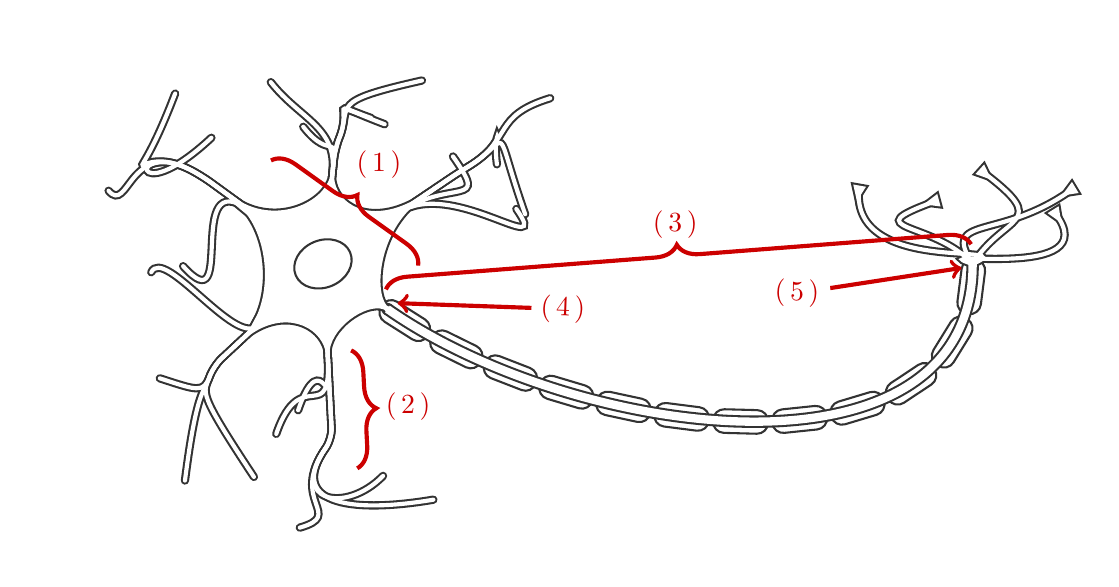
\begin{tikzpicture}[
        scale = 1.5,
        draw = black!80,
        fill = white,
        ]
    
    \clip[use as bounding box] (-2.5,-2.5) rectangle (6.5,2);
    %\draw[help lines] (-2.5,-3) grid (6,2);
    %\draw[white,->] (0,-4) -- (0,4);
    %\draw[white,->] (-3,0) -- (6,0);
    
    % Random Num shit
    \def\ranAngle#1{\pgfmathrandominteger{#1}{-75}{75}}
    \def\ranLength#1{\pgfmathrandominteger{#1}{5}{15}}
    \def\ranScale#1{\pgfmathrandominteger{#1}{-10}{10}}

    % Colors
    \def\clr{black!80}

    
    % Random number generation seed
    %\def\seed{220699}
    %\def\seed{04081999}
    \def\seed{1669}
    %\def\seed{1984}
    %\def\seed{2356}
    \pgfmathsetseed{\seed}
    
    % Various constants
    \def\sh{5.0}                    %
    \def\w{8.0}                     %
    \def\bloatStr{0.5}              %
    %\def\armLen{1}                  %
    %\ranLength{\armLen}             %
    %\def\pole{0.5}                  %
    \ranLength{\pole}               %
    \def\axonLen{5.5}               %
    \def\tentLen{1/15}              %
    \def\c{0.1}                     %
    \def\rx{0.25}                   %
    \def\ry{0.20}                   %
    \def\angle{45}                  %
    \def\linthicc{3pt}              %
    \def\linthic{0.5*\linthicc}     %
    \def\linthin{0.5*\linthic}      %

    
    % Angles for the polar coordinates, uses degrees for god knows what reason
    %\pgfmathrandominteger{\rara}{0}{300}
    \pgfmathsetmacro{\pI}{34}
    \pgfmathsetmacro{\pII}{84}
    \pgfmathsetmacro{\pIII}{144}
    \pgfmathsetmacro{\pIV}{223}
    \pgfmathsetmacro{\pV}{273}
    \pgfmathsetmacro{\pVI}{325}

    % Shortcut for loop
    \def\forlist#1{
    \foreach \i in {\pI,\pII,\pIII,\pIV,\pV,\pVI}{
                    #1
                    }
            }
    
    % Fixed points
    \coordinate (O) at (0,0); % The origin
    \coordinate (SC) at (\axonLen, 0.0); % The synaptic cleft potistion

    % Some custom commands/shortcuts
    % Cell "spikes"
    \def\pcoord#1#2{{#1:#2}}
    \forlist{
        \pgfmathrandominteger{\armLen}{10}{15}
        \coordinate (P\i) at (\pcoord{\i}{\armLen/15});
        %\fill (P\i) circle (1.5pt);
        }
    \coordinate (P\pVI) at (\pcoord{\pVI}{2/3});
    \coordinate (AH) at (P\pVI);


    \def\bloat#1{{#1:\bloatStr}}
        \def\contr#1#2{(P#1) .. controls (\bloat{#1+\sh}) and (\bloat{#2-\sh}) .. }
    \def\aggcontr#1#2#3#4#5{
                \contr{#1}{#2}
                \contr{#2}{#3}
                \contr{#3}{#4}
                \contr{#4}{#5}
                }
    \def\axonPath{(P\pVI) to[out=\pVI, in=-90] (SC)}
    \path foreach \SIGN/\i in {-/1, +/2}{
        \axonPath -- ([turn]\SIGN 45:0.75) coordinate (CL\i)};

    % Axon mylene sheath decoration
    \begin{scope}[decoration={markings,
                    mark=between positions 0.03 and 1 step 0.75cm
                    with { \node   [rectangle, 
                                    rounded corners, 
                                    fill = white, 
                                    draw = \clr,
                                    inner sep=0pt,
                                    minimum height=0.30cm,minimum width=0.7cm,
                                    behind path,
                                    %scale = 0.5,
                                    transform shape] {};}}]
        \draw[postaction={decorate}, line width = 0.75pt]
            \axonPath;
    \end{scope}


    \def\synCleft{
    \foreach \i in {-0.3,-0.15,0.4,0.8,1.4}{
        \pgfmathrandominteger{\slp}{-4}{12}
        \ranAngle{\srpI}
        \ranAngle{\srpII}

        \def\tmp{90+\srpI}
        \draw[line cap = butt] ($(CL1)!\i!(CL2)$)+(95:\slp/20) node[fill, draw, scale = 0.20, isosceles triangle, rotate = {-\tmp}] {} .. controls +(180+95+\srpI:0.75) and +(95+\srpII:0.5)  .. (SC);
    }}


        
                    
        % Cell body
        % gives the juicy looking cell body
        % Generates random angles for the branching arms
        \def\limbConstruct{
            \ranAngle{\ra}
            \ranAngle{\rb}
            \ranAngle{\rc}
            \ranAngle{\rangA}
            \ranAngle{\rangB}
            \ranAngle{\rangC}
            \ranLength{\rla}
            \ranLength{\rlb}
            \ranLength{\rlc}
            \ranLength{\rext}
            \ranLength{\rarm}
            
            \foreach \v in {\ra:\tentLen*\rla,
                            \rb:\tentLen*\rlb,
                            \rc:\tentLen*\rlc
                            }{
                \draw [line cap = round, rounded corners]
                    (P\i) -- ([turn]0:\rext/20) 
                    .. controls 
                    ([turn]\rangB :\rarm/20) and 
                    ([turn]\rangC:\rarm/20) .. 
                    %to[out=\rangB, in=\rangC]
                    ([turn]\v) 
                    %node[ draw, isosceles triangle, rotate = \rangC, scale = 1]{}
                    ;
                }
            \foreach \v in {\i+\rb:\tentLen*\rlc,
                            \i+\rc:\tentLen*\rla
                            }{
                \draw [line cap = round, rounded corners]
                    (PP\i) 
                    .. controls 
                    ([turn]0:\rarm/20) and 
                    +(\rangA:\rarm/20)  .. ([turn]\v) 
                    %node[fill,draw, isosceles triangle, rotate = 180+\rangA, scale = 0.00005]{}
                    ;
                }}

        % Builds and outlines the Neuron
    \foreach \COLOR/\THICKNESS in {black!80/\linthicc, white/\linthic}{
        \begin{scope}[line width = \THICKNESS, \COLOR ]
                    
            \pgfmathsetseed{\seed}
            \foreach \i in {\pI,\pII,\pIII,\pIV,\pV}{
                \draw 
                    (P\i) -- (\i:\pole/13) coordinate (PP\i);
                    
                \limbConstruct
                }
            
            \filldraw  
                \aggcontr{\pI}{\pII}{\pIII}{\pIV}{\pV} 
                (P\pV) .. controls (\bloat{\pV+\sh}) and (\bloat{\pVI}) ..              
                (P\pVI) .. controls (\bloat{\pVI}) and (\bloat{\pI-\sh}) ..
                cycle;

            \ifx\clr\COLOR
            \draw [line width = 1.5*\linthicc]
                \axonPath;
            \fill (P\pVI) circle (\linthic);
            \else 
            \draw [line width = \linthicc]
                \axonPath;
            \fill (P\pVI) circle (\linthin);
            \fi
            
            \synCleft
            \end{scope}
    }


    \draw[rounded corners, rotate = 23, line width = \linthin]  
            (0,0) ellipse [x radius=\rx cm, y radius=\ry cm];
    %\draw[white,rounded corners, rotate = 90]  
    %        (45:\rx) rectangle (225:\rx);

    % Labeling
    \begin{scope}[opacity = 1, red!80!black, line width = 1.5pt]
        
        % Soma label
        \pgfmathsetmacro{\somaSlope}{(\pIII + \pVI)/2}
        \path (P\pIII) -- +(\somaSlope:-0.45) coordinate (Sa);
        \path (P\pVI)  -- +(\somaSlope:-0.45) coordinate (Sb);
    
        \pgfmathsetmacro{\somaTextSlope}{\somaSlope + 90}
        \draw[decoration ={brace, amplitude = 8}, decorate] 
            (Sa) -- (Sb) node[midway, sloped, allow upside down= true, 
            above, yshift = 0.3cm] { \rotatebox{-\somaTextSlope}{$\left(\, 1 \,\right)$}};

        % Dendrite label
        \path (P\pV) -- ++(0:0.20) coordinate (Da);

        \draw[decoration ={brace, amplitude = 8}, decorate] 
                (Da) -- ($(Da)!1!(Da)+(\pV:1)$) 
                node[midway, sloped, 
                above, yshift = 0.25cm, allow upside down= true] { \rotatebox{-\pV}{$\left(\, 2 \,\right)$} };

        % Axon label
        \pgfmathsetmacro{\axonTextSlope}{ atan2( (11/15) * sin(\pVI), \axonLen * cos(0)) }
        \draw[decoration ={brace,amplitude = 8, raise = 0.25cm}, decorate] 
                (P\pVI) -- (SC) node[midway, sloped, 
                above, yshift = 0.45cm] {\rotatebox{\axonTextSlope}{$\left(\, 3 \,\right)$}};    
        
        % Axon Hill label
        \draw[<-] 
                (AH)+(30:1mm) node (AHpoint) [circle] {} -- +(0:1.5) node[align=left, pos = 0.99, sloped, 
                fill = white] {\rotatebox{0}{$\left(\, 4 \,\right)$}};   

        % Synaptic Cleft label
        \pgfmathsetmacro{\axonTerminalTextSlope}{pi/2 *((4 - \axonLen)/(-0.25 - 0.0))}
        \draw[<-] 
                (SC)+(200:1mm) node (SCpoint) [circle] {} -- (4,-0.25) node[align=left, pos = 0.99, sloped, 
                fill = white] {\rotatebox{-\axonTerminalTextSlope}{$\left(\, 5 \,\right)$}};   
    \end{scope}

    %\draw (-10,0) to (10,0);
    %\draw[yshift = 0.25cm] (-10,0) to (10,0);
\end{tikzpicture}     

\end{document}